\chapter{Implementation}
\label{cha:implementation}

This chapter describes which technologies can be used to implement BGE and how a model realisation of the BGE modules can look like. A prototype is available on \newline \textit{http://games.fkmt.de}. 

Currently implemented BGs on this instance are the \textit{beergame} \cite{beergame}, \textit{SaltSeller} \cite{saltseller}, SaltSeller for many players (with a simplified market model), the example game from the BMDL paper \cite{bmdl1}, the \textit{oligopoly game} as well as \textit{stone-paper-scissors}. The game code of the beergame and of stone-paper-scissors is included in the appendix.
\begin{figure}[t]
	\centering
	\includegraphics[scale=0.58]{figures/architecture.png}
	\caption{BGE architecture overview}
	\label{fig:arch}
\end{figure}

\section{Choice of technology}
\label{sec:imp:technology}

Figure \ref{fig:arch} provides an architecture overview of this implementation of BGE. The following sections describe in detail which technologies are being used and for what reason this is done.

\subsection{BGD object model}
\label{sub:imp:BGD}

The first question to arise is the choice of the object-oriented programming language that is used to implement BGD. Recalling the UML diagram from figure \ref{fig:uml} it is obvious that its most straightforward implementation contains a lot of dynamic types:
\begin{itemize}
\item The type of (function)parameters and attributes or the return type are often decided only at runtime, depending on the game which is currently played. A (game)parameter for instance might be a string or a numerical value and the return type of the \newline $getParameter()$ method is consequently either a string or a number.
\item Some functions accept optional parameters as for example an optional Chart object.
\item Some objects must be extended at runtime. The content of the Round object for example is entirely dependent on the game that is currently played.
\end{itemize}
As conclusion it seems advisable to refrain from using a static programming language such as Java, C or C\# and to prefer a scripting language such as Perl, Python or JavaScript. In addition, all of these three scripting languages natively support first-class functions which facilitates the implementation as seen in section \ref{subsub:variables}.

 The success of a BGE implementation depends on whether the platform can be deployed securely without posing potential risks to the server. The list of security measures from section \ref{subsub:security} in order to run untrusted code on the server is neither complete nor easy to achieve. As a consequence, the second option of running all untrusted code in the browser is preferred. This has also the advantage that the server becomes a mere orchestrator and that the clients take all the load for the calculation of the games' market models. JavaScript being natively supported by all browsers is therefore the favoured programming language for this BGD implementation and taken as assumption for the remaining part of this chapter.
 
\subsection{Client-server-communication: the WebSocket Protocol}
\label{sub:imp:cs}

In a multiplayer BG a great deal of realtime synchronization must take place between the server and the participating players/clients. An implementation with client-side game code execution must support at least the following communication steps:
\begin{itemize}
\item A client must be able to request to play a certain game.
\item The server must join clients together who want to play the same game and inform the players to either wait for other players or to start the game if a sufficient number of players has been reached.
\item The players submit input decisions or questionnaire answers to the server.
\item The server must collect these inputs and redistribute them to the clients for output-calculation after all players have submitted their inputs. 
\item If a player does not answer within the maximal decision time or leaves the game before it has finished the server must disconnect this client, record the abort and use default input values for this player for the rounds to come.
\item The clients must submit their output calculation results after each round or at least at the end of the game so that the server can store the game history to the database.
\end{itemize}

The type of communication channel between client and server over the internet is defined by a communication protocol supported by the browser as well as by the server. Communication protocols are part of the application layer of the OSI model and rely on transport protocols such as TCP or UDP. 

HTTP is a frequently used communication protocol in the internet. Here, any message or data or response from the server must be triggered by a request from the client. The communication is uni-directional since a given instance of HTTP cannot be used to send data in both directions, but only from the client to the server or the other way around.

Previous experiences of implementing a multiplayer BG \cite{saltseller} have shown that using HTTP for communication and synchronization between server and clients leads to a rather complex implementation. The game and the round objects must know different states. A round may for example know the states \textit{running} and \textit{done} depending on whether some or all inputs have been submitted by the players. Depending on the combination of the current game state and round state different actions must be taken (e.g.~calculate outputs if all inputs are submitted) and a certain html page must be rendered or the HTTP request must be redirected to the same or to another location.

Since every communication in HTTP must be initiated by the client, each client must send a HTTP AJAX request in a fixed interval (e.g.~each second) checking the new game and round state, which is called HTTP polling. Assuming there are two players A and B. If A has already submitted its input value but B has not done yet, the last round state A knows is \textit{running}. After B has also submitted its input the round state changes to \textit{done} and A sees with a maximal delay of one second that its own round state and the true round state are different. This triggers a reload of the page and the new state combination leads to some action, in this case maybe the calculation of the outputs and the rendering of a result page.

As a summary, the use of HTTP in \cite{saltseller} led to
\begin{itemize}
\item network overhead for HTTP polling, where a better multiplayer synchronization (with a smaller polling interval) results in bigger overhead,
\item a bad user experience due to page reloads,
\item a highly complex code with many HTTP redirects and different state combinations.
\end{itemize}

A lot would be gained if the server could also initiate the communication and for example inform its clients that all inputs have been submitted. Such a behaviour can be realised for instance using the WebSocket Protocol \cite{websocket} which has been introduced in 2011 and which is now implemented in all major browsers. It establishes a full-duplex (bi-directional) communication channel between server and client through which both can send data at any time.

As a main advantage, the WebSocket Protocol significantly facilitates the implementation of the necessary communication steps. It is used for that reason as communication protocol within the playing environment of BGE. All other environments do not need sophisticated synchronization between server and clients, they only load resources from the server. HTTP was built for that use case and is therefore used in all other environments except the playing environment. The following part of this section describes the specification of the WebSocket Protocol.

In inter-process communication (IPC), sockets are the endpoints of a communication channel on which both processes can send and receive data. Inter-process communication between two processes on different machines can be established over a computer network such as the internet. An internet socket is defined by the unique internet address of the machine (IP address), the delivery slot of this instance of communication (port number) and a the name of the transport protocol used (e.g. TCP or UDP), since different protocols can use the same port \cite{bsd}.

Web browsers do not allow to establish a raw communication channel based on e.g. TCP because this would allow malicious scripts to attack various services on the internet listening on such a connection which are not prepared to deal with harmful input. WebSockets add a layer on top of TCP enabling such a bi-directional communication channel between two processes that are explicitly prepared for it. 

For that reason the protocol specifies an URI-based addressing mechanism\footnote{"ws/wss:" "//" host [ ":" port ] path [ "?" query ]}, for example \textit{wss://server.example.com/secureChat}. Therefore, a WebSocket connection is identified by a scheme component (ws or wss for a TLS secured connection), a host, a port (optional, defaults to 80/443) and a resource (optional, consists of path and/or query). Since several hosts can be hosted one one machine and since it is possible to specify a resource this implies that multiple WebSocket services can share one port and/or one IP address \cite{websocket}. 

In order to establish a WebSocket connection the client and the server must perform the WebSocket handshake. WebSockets use TCP and can be optionally secured with TLS. The client initialises the handshake with a HTTP GET request with Upgrade header. Using HTTP and not another protocol for the handshake allows the WebSocket protocol to coexist with the existing HTTP infrastructure sharing port 80/443 with HTTP clients [Ibid.]. 

In order to establish a WebSocket connection with the chat service mentioned above, a client would open a TLS connection to \textit{sever.example.com} and send a HTTPS GET request for the resource~\textit{\textbackslash secureChat}. Among others this request must specify the Upgrade, Host \textit{(server.example.com)}, Origin \textit{(api.mallory.com)} and Sec-WebSocket-Key Headers. The \textit{Origin} Header field is set by the browser indicating the origin of the script trying to access the service. Typically, a server could only allow trusted scripts e.g. from \textit{example.com} in the example above and reject an unknown script from \textit{mallory.com}. This does not replace authentication or input validation because non-browser clients can also establish the WebSocket connection and can easily fake the Origin header [Ibid.]. 

\textit{Sec-WebSocket-Key} is a base64-encoded 16 byte nonce which the server must concatenate with a predefined GUID. If he accepts the client's connection he must send a HTTP response with status code 101 (Switching Protocols) which includes the \textit{Sec-WebSocket-Accept} Header containing the hashed value. The WebSocket connection cannot be established if this value doesn't correspond with the expected value. With this mechanism the server has to prove that he has received and understood the client's handshake accepting only WebSocket connections. This prevents an attacker to send a message over another protocol as e.g. HTTP that looks like a WebSocket message [Ibid.]. It also prevents from tricking non-WebSocket servers to echo a valid WebSocket handshake response in order to establish an unauthorised connection\footnote{http://www.ietf.org/mail-archive/web/hybi/current/msg06551.html, retrieved on 28 Jan. 2016} \footnote{http://www.ietf.org/mail-archive/web/hybi/current/msg01198.html, retrieved on 28 Jan. 2016}.

After the WebSocket connection has been established both server and client can send and receive data which must be framed as specified by the base framing protocol [Ibid.]. Frames may be fragmented which means that the payload data can be splitted into several frames. This has the advantage that intermediaries who know the protocol and which have seen the handshake can do fragmentation according to network needs. It also implies that both client and server can start to send a message before knowing its size and thus do not have to buffer it completely before sending it. Among others, a frame specifies the content type (text, binary, reserved, control frame or continuation of a fragment), the payload length and an optional masking key. 

Clients must always mask every frame with a new 32 bit random nonce which is unpredictable from within the end application providing the data. Servers must never mask a frame. If one party violates this rules, the connection must be closed. The idea behind is that the client application cannot predict how the data appears on the wire. Otherwise there is a chance that cache poisoning attacks can be leveraged on transparent proxies which are often used for example in enterprise networks to cache content \cite{hack}. In some cases, such intermediaries do not properly implement the HTTP Upgrade mechanism causing the WebSocket handshake to succeed while still interpreting the following traffic as HTTP traffic. If an attacking script is then able to predict how the sent data appears on the wire it can send a WebSocket message to an attacking server which looks like a valid HTTP GET request which is for example fetching a script such as \textit{Google Analytics} with the host \textit{google.com}. The server will then send a response containing a compromised script. For the proxy this looks like a valid response from Google and he now caches the compromised script instead of the real one. All users of the proxy requesting Google Analytics will then receive this compromised script instead of the real Google Analytics.


\subsection{Server-side JavaScript}
\label{sub:imp:server}

WebSocket implementations are available for all server-side technologies such as Java EE, .Net, Python or PHP. However, the event-like character of a WebSocket connection seems to be well suited for JavaScript's event-based, asynchronous execution model. 

\subsubsection{Asynchronous execution model of JavaScript}
\label{sub:sub:async}

In the browser, when performing an I/O operations such as requesting remote content via an AJAX call, or when waiting for an user interaction or setting a timeout, JavaScript does not block the process and does not wait for the operation to complete, but continues to run other code that follows next. As soon as the server delivers the content or the user clicks a button or the timer has run down, the code associated with the operation is executed. Listing \ref{lst:javascript} demonstrates this behaviour for a programme that asynchronously fetches the HTML content of a website using the jQuery library.

\begin{lstlisting}[language=Javascript, caption=JavaScript's asynchronous execution model, label=lst:javascript]
jQuery.get('http://games.fkmt.de', callback); // AJAX call
function callback(data) {
    console.log(data); // Prints the HTML content of the requested website 
}
var pi = calculatePi(1000000); // Calculates Pi with 1M decimal places
console.log('Done. Pi = ' + pi); // Prints "Done. Pi = 3.14..."
\end{lstlisting}
In most programming languages which use a synchronous execution model, a similar programme would wait for the response from the requested website and then print its HTML content on the standard output. After that it would  start calculating Pi and finally print \textit{Done. Pi = 3,14...} Hovewer, the JavaScript programme from listing \ref{lst:javascript} behaves differently. In the first line, the HTTP GET request function gets executed with a callback function passed to it as second parameter. Next, the calculation of Pi is immediately started, without waiting for the network to respond. \textit{Done. Pi = 3,14...} gets printed on the standard output as soon as the result has been calculated. If in the meantime the network has delivered, the callback function is executed and the HTML content is printed. Otherwise the callback function printing HTML will be executed as soon as the network responds.

The JavaScript engine achieves this non-blocking behaviour for I/O and other asynchronous operations using a call stack (also referred to as execution stack or just stack), a message queue and an event loop\footnote{http://2014.jsconf.eu/speakers/philip-roberts-what-the-heck-is-the-event-loop-anyway.html, retrieved on 25 Jan. 2016} \footnote{https://developer.mozilla.org/en-US/docs/Web/JavaScript/EventLoop, retrieved on 20 Dec. 2015}. Messages (events) with an associated callback function get enqueued in response to external events, such as a user clicking a button or a response arriving from a HTTP request. The event loop continuously polls the queue for the next message and puts the associated callback function on the call stack if and only if it finds the stack empty.

Running the file\footnote{In the browser, we cannot just read from a file but would typically embed this program in a <script></script> tag of a html file.} containing the example above, the first function to be put on the call stack is an implicit \textit{eval()} function containing all the code from the file, which is similar to the \textit{main()} function in C or in C-derived languages. Next, the \textit{jQuery.get()} function is put on top of that. It calls the \textit{open()} and \textit{send()} functions from the browser-dependant implementation of the XMLHttpRequest\footnote{https://www.w3.org/TR/XMLHttpRequest/, retrieved on 25 Jan. 2016 } Web API\footnote{https://developer.mozilla.org/en/docs/Web/API, retrieved on 25 Jan. 2016}, which is typically implemented in C(++) as part of the browser's rendering engine and which runs separated from the JavaScript engine in another thread of the browser process. The XMLHttpRequest implementation is from now on in charge for sending the HTTP GET request to \textit{http://games.fkmt.de} and waiting for the response, which results in removing all corresponding function calls from the stack of the JavaScript engine and adding it to the stack of the rendering engine. At an unknown time in future, when the response from the network is available, the rendering engine enqueues the callback associated with this event of the available response in the message queue of the JavaScript engine. If and only if its call stack is then empty, the callback function will be put on the call stack by the event loop, which is continuously waiting for new events to arrive.  

In the meantime, immediately after calling \textit{jQuery.get()}, \textit{calculatePi(1000000)} is put on the stack starting its calculation. After it returns, the result is printed on the standard output (the Browser's console). The call stack is now empty since the end of the file has been reached, which means the implicit \textit{eval()} function can be taken from stack as well. The event loop of the JavaScript engine then continuously polls the message queue for the next event that has been enqueued in the past or that will be enqueued in the future and puts its associated callback on the stack and then pauses polling until the stack is empty again. In the example above, this results in printing the HTML content of the requested website on the standard output.


\subsubsection{JavaScript on the server: Node.js}
\label{sub:sub:node}

JavaScript is omnipresent as scripting language in web browsers, but its deployment on server-side is quite new. Ryan Dahl introduced Node.js in 2009 as a "purely evented, non-blocking infrastructure to script highly concurrent programs"\footnote{https://www.youtube.com/watch?v=ztspvPYybIY, retrieved on 03 Apr. 2016}. Thus, the main idea behind Node.js is to provide the programmer with a server-side environment where all I/O (file system, network, IPC, timers...) can only be done in a non-blocking, asynchronous way. For that, Node.js uses the same concepts as a JavaScript engine, which are an event loop and one single execution stack.

In contrast to for example an Apache web server running a PHP or a Java application, Node.js serves all clients within a single thread. This would not be possible if an I/O operations such as querying the database from one request would block the other requests from being served. This is why all I/O in Node.js is non-blocking. If client A requests something from the server's database, which is in computational terms a very slow operation and takes millions of CPU clock cycles, Node will go on serving requests from other clients and call the callback function associated with A's request as soon as the content from the database is available. 

In the conventional synchronous execution model, each client's request is executed in a new thread since a slow database operation would otherwise block the other clients from being served. Since each new thread consumes a little of the server's memory and the context switching also needs some CPU time, the asynchronous model is well-suited to build scalable web applications which can serve a lot of concurrent connections. The developer need not be experienced with complex (thread-related) tasks such as synchronizing resources since each callback is finished and hence all of its function calls have disappeared from the stack before another one is polled by the event loop. It can thus be used to create efficient applications with comparably little effort. Certainly, CPU-intensive tasks such as the calculation of Pi in listing \ref{lst:javascript} block such a single-threaded setting and must be either avoided or additional child processes or clusters must be spawned \cite{nodedoc}, which might make implementations again more difficult.

\begin{figure}
	\centering
	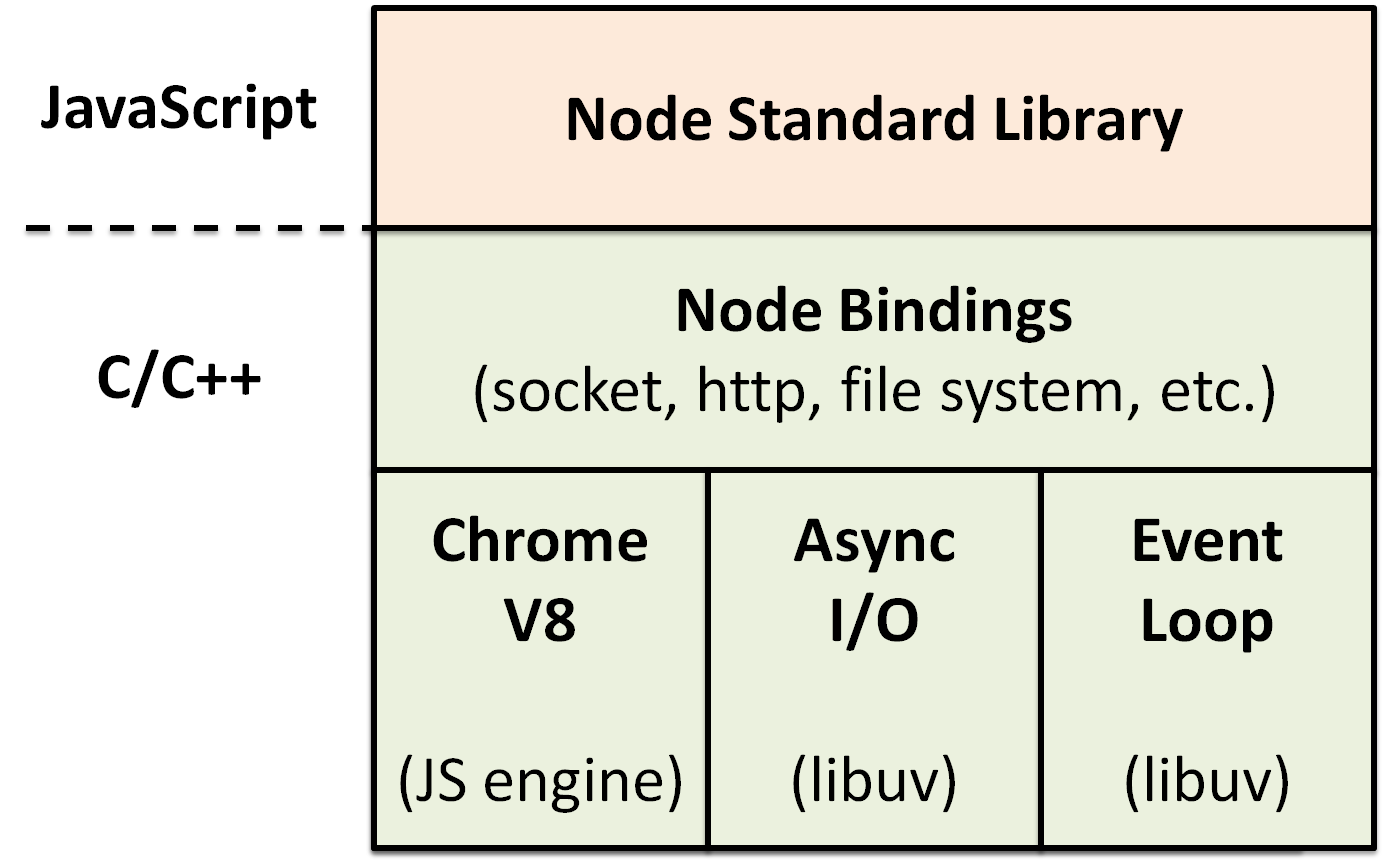
\includegraphics[scale=0.5]{figures/node.png}
	\caption{Node.js architecture overview. Source: stackoverflow.com/questions/36491385}
	\label{fig:node}
\end{figure}
Figure \ref{fig:node} shows an overview of the architecture of Node.js. The API\footnote{https://nodejs.org/api/, retrieved on 04 Apr. 2016} (Standard Library) of Node.js is written in JavaScript and enables the programmer among others to access lower level functionality of the operating system via JavaScript. It is split into different (core) modules providing built-in support for HTTP, TCP, UDP, DNS, TLS, filesystem access, Processes, Buffers, Streams, Events and more. Apart from the core modules, the programmer can import from a large number of other open-source modules via the node package manager (NPM), which has grown the world's largest ecosystem for open-source libraries\footnote{https://www.npmjs.com, retrieved on 04 Apr. 2016}. 

All other parts than Node's API are written in C or in C++. Node.js is built upon Google's JavaScript engine V8. One one hand, V8 is responsible for parsing the user's JavaScript programs and translating it to machine code. On the other hand, V8 provides the Runtime environment, bridging native C++ functions and objects into JavaScript objects. Like this, it is possible to "wrap C++ functions and data structures within JavaScript objects so that they can be manipulated by JavaScript scripts"\footnote{https://developers.google.com/v8/embed\#templates, retrieved on 19 Apr. 2016}. Node.js uses V8 Object and Function Templates to achieve this behaviour. Browsers using V8 apply the same concept in order to expose native implementations of DOM, XMLHttpRequest or other Web APIs to JavaScript and make them available for example as the global \textit{Window} object. 

In Node, most modules of the API have a native C++ counterpart (Node Bindings) providing the actual functionality. For example, the \textit{fs} module in \textit{lib/fs.js} of the API is bound to \textit{src/node\_file.cc} where file system related functionality such as open, read, write, stat and so on can be found. 

However, Node's design goal is to provide purely asynchronous, non-blocking I/O. For example on the network or the file system, asynchronous means that an application expresses interest in a remote resource or a file at one point and uses the data at a different point of time and (memory) space. Non-blocking means that the process was free to do other tasks in the meantime. In UNIX, regular file system I/O is always blocking, while it might be blocking or non blocking in Windows, using a different mechanism\footnote{http://tinyclouds.org/iocp-links.html, retrieved on 08 Apr. 2016}. For asynchronous operations on network sockets, different operating systems provide different system calls\footnote{https://banu.com/blog/2/how-to-use-epoll-a-complete-example-in-c/, retrieved on 08 Apr. 3016}. Node.js and other projects use the C-library \textit{Libuv} in order to realise asynchronous, non-blocking I/O on all major operating systems. It implements an event loop and uses the same callback pattern as JavaScript in order to notify about an incoming event\footnote{http://nikhilm.github.io/uvbook/basics.html, retrieved on 08 Apr. 3016} as well as in order to specify the application logic connected to that certain event. Libuv was created as part of the Node.js project as a replacement for \textit{Libev} when Node was to be ported to Windows. It can be described as a unified interface for asynchronous I/O on all major operating systems. It tries to use the most efficient, non-blocking functionality that each operating system provides for each different type of I/O. When there is no such functionality at all, as for example with file system I/O in UNIX, Libuv uses a thread pool in order to emulate non-blocking behaviour. 

An example: Listing \ref{lst:libuv} shows a simple program that asynchronously reads from a file on the file system, calling Libuv's \textit{uv\_fs\_open()} and \textit{uv\_fs\_read()} functions. Both functions are passed among others a pointer to the event loop, a request object and a callback function. Libuv uses request objects to preserve the context between starting an asynchronous operation and its callback. Thus, the request object is later passed to the callback as parameter. For the rest of this example, the two callbacks are named \textit{on\_open} and \textit{on\_read}. 
\begin{description}
\item[Open.] The \textit{uv\_fs\_open()} call is also passed a path to the file to be opened. Libuv then calls the \textit{open()}\footnote{http://man7.org/linux/man-pages/man2/open.2.html, retrieved on 24 Apr. 2016} facility of the operating system the example program is executed on. If this can be done only in a blocking way, such as on UNIX, Libuv gives this task to a thread pool. Many CPU cycles later, the file system responds with a file descriptor. Libuv then writes this file descriptor to the request object and calls \textit{on\_open}, passing it the request object as parameter. Since the example program is supposed to read from a file, \textit{on\_open } calls \textit{uv\_fs\_read()}, passing it the file descriptor representing the file to read from.
\item[Read.] The \textit{uv\_fs\_read()} call is also passed a buffer. Libuv calls the corresponding \textit{read()} system call\footnote{http://man7.org/linux/man-pages/man2/read.2.html, retrieved on 24 Apr. 2016}, which writes into the buffer. Again, a thread pool is used if necessary. After the data has been read, Libuv writes the number of read bytes to the request object and calls \textit{on\_read} with the request object as parameter.
\end{description}

The event loop and thus a whole Libuv program run as long as there are events to watch out for. The simple example program from listing \ref{lst:libuv} terminates after the open and read have finished. This is described by the two short-lived request objects that preserve the context between start and end of the asynchronous operations. In more elaborate examples, a request represents an asynchronous operation on a long-lived \textit{handle} object. Handles are used to express interests in events on I/O devices, processes or timers. Examples would be a handle on a TCP socket (e.g. for writing a server) or a handle on a pipe (e.g. for streaming from/into a file or for inter-process communication). In this case, the event loop terminates after the socket or the pipe have been closed. 

\begin{lstlisting}[language=C, caption=Libuv example program. \newline Based on https://github.com/nikhilm/uvbook/tree/master/code/uvcat, label=lst:libuv,float,floatplacement=H]
... // Other includes
#include <uv.h> // Include Libuv
static char buffer[1024];
static uv_buf_t uv_buffer;
uv_fs_t open_request; // Create two request objects
uv_fs_t read_request;
void on_read(uv_fs_t *request) {
    fprintf(stdout, "The read data: %s\n", uv_buffer.base);
    fprintf(stdout, "Number of bytes read: %i\n", request->result);
}
void on_open(uv_fs_t *request) {
    uv_buffer = uv_buf_init(buffer, sizeof(buffer));
    uv_fs_read(uv_default_loop(), &read_request,
               *request->result, // Contains the file descriptor
               uv_buffer, ... , on_read);
}
// argv[1] contains the file path
int main(int argc, char **argv) {
    uv_fs_open(uv_default_loop(), &open_request, argv[1], ... , on_open);
    uv_run(uv_default_loop(), UV_RUN_DEFAULT); // Runs the event loop
}
\end{lstlisting}

Recalling figure \ref{fig:node}, how is Libuv to be integrated into the architecture of Node.js? The Node Bindings embed V8 and use it to expose Libuv's functionality to the JavaScript API. Listing \ref{lst:node} translates the C-program from listing \ref{lst:libuv} into a (ES6) JavaScript program. After saving its content to a file named for example \textit{readfile.js}, the program can be executed with the command \textit{node readfile.js /path/to/file}. This will
\begin{itemize}
    \item create a new V8 instance,
    \item create a C++ Process object,
    \item expose this object with V8 as the blueprint for the global \textit{process} object of the Node API\footnote{https://nodejs.org/api/process.html, retrieved on 25 Apr. 2016}, 
    \item additionally add a function called \textit{binding()} to the process object, which is not described in the API but which allows JS code to access the C++ Bindings (this is used in the API core modules), 
    \item make V8 compile and run the startup script in \textit{src/node.js} passing it the process object,
    \item let the startup script install global objects and functions and the module loader in the user space, the latter enabling \textit{require(moduleName)} to load the corresponding (core) module from the API,
    \item read the content of \textit{readfile.js} and run it,
    \item due to \textit{require('fs')} in the source code: load the file system core module and call its \textit{read()} and \textit{open()} functions,
    \item via \textit{process.binding('fs')}, the file system core module calls Read() and Open() from the C++ Bindings,
    \item these functions call Libuv's \textit{uf\_fs\_open()} and \textit{uv\_fs\_read()}, create two request objects and install the callbacks,
    \item start Libuv's event loop calling \textit{uv\_run()} and loop as long for incoming events as there are active handles or requests.
\end{itemize}


\begin{lstlisting}[language=Javascript, caption=Example program in JavaScript using Node.js., label=lst:node]
'use strict';
const fs = require('fs'); // Load the file system core module
fs.open(process.argv[1], 'r', (err, fd)=> { // Arrow functions: ES6
// (err, fd)=> { ... } is here the same as function(err, fd) { ... }
    const buf = Buffer.alloc(1024); // Safe buffer alloc (Node v.5.10.1+)
    fs.read(fd, buf, 0, 1024, null, (err, bytesRead, buffer)=> {
        console.log('The read data: ', buffer.toString('utf8'));
        console.log('Number of bytes read: ', bytesRead);
    });
});
\end{lstlisting}

 \subsubsection{The big picture: Two event loops and WebSockets}
\label{sub:sub:bigpicture}

WebSockets, as stated at the beginning of this chapter, fit perfectly into the asynchronous, event-based execution model of JavaScript and Node.js. Both server and client can send an event, which is nothing more than a string, together with payload data at any time of the connection to the other side. Here, a listener must be defined for that specific event specifying a callback function. Whenever this specific event is sent, the listener is aware of the listened event and executes a callback function with the payload data passed as parameter. 
Table \ref{tab:engine} in the next chapter specifies the concrete events and payload data that are used for the playing environment.

Figure \ref{fig:loops} summarises the main idea of this BGE implementation: Architecture-wide use of the expressive JavaScript programming language and of event-driven, asynchronous programming. WebSockets, needed for the complex synchronisation in the playing environment, fit seamlessly into that concept. 

\begin{figure}[ht]
	\centering
	\includegraphics[scale=0.6]{figures/loops.png}
	\caption{BGE architecture: Two event loops and WebSockets.}
	\label{fig:loops}
\end{figure}

Following this reasoning, Node.js is seen to be an ideal server-side technology for the implementation of BGE. The WebSocket library \textit{Socket.io}\footnote{http://socket.io/, retrieved on 6 Dec. 2015} is very easy to use and drastically simplifies realtime synchronizations between server and clients. The web server realised with the framework \textit{Express}\footnote{http://expressjs.com/, retrieved on 6 Dec. 2015} in combination with the command-line tool \textit{forever}\footnote{https://github.com/foreverjs/forever/, retrieved on 6 Dec. 2015} proved to be sufficient for setting up and maintaining the architecture on a Linux server with very limited physical resources.

Yet the main reason for choosing Node.js was another. Using JavaScript on the server significantly facilitates the development process and maintains a very high flexibility since both client and server speak the same language. In the beginning it was for example considered to execute game code on the server-side. After the security measures from section \ref{subsub:security} turned out to be very hard to realise, the already existing BGE code could be shifted to the client without having to change anything. With Node.js, native JavaScript objects such as the whole Game object serialised as JSON become the data exchange format between server and client. This is -- especially in combination with WebSockets -- a very powerful feature. Sending an object over the internet at any point in the program code and in any direction becomes almost as simple as calling a function.

\subsection{NoSQL Database}

HTTP is a stateless protocol. Due to this fact the database played a central role in the HTTP implementation of the SaltSeller business game \cite{saltseller}. Whenever some change occurred, as for example the calculation of a round's outputs or the game-abort of some player, this change needed to be written to the database. The next HTTP request then fetched the newest state from the database and kept on working with that. Especially when such a system has to serve a lot of games simultaneously, such a frequent database access might become a performance issue.

The WebSocket Protocol is stateful, which means that the connection between server and client is persistent until the client closes or refreshes the tab or redirects or gets redirected to another HTML page. The use case of WebSockets should therefore be well considered since establishing such a connection needs more resources than establishing a HTTP connection. 

For the playing environment of BGE it is indeed worth that effort. Apart from the much simpler implementation, the database becomes a backup tool for later game data analysis rather than a system critical component. In this implementation of BGE, where all calculations are performed by the clients, the game object is initialised on the client side and grows as the game evolves (section \ref{sec:bge}). Only after the game has finished the clients transmit the Game object, now containing the complete game history, to the server, where it gets written to the database. The number of database accesses thus significantly decreases, improving the performance of the architecture.

In consequence, performance indicators such as transactions per second or the maximum number of records that can be stored need not play a major role for the choice of a database technology. Even if a lot of games are played simultaneously the database is unlikely to become the bottleneck of the architecture. 

Much more important are the costs or the effort for saving JavaScript JSON objects. Relational databases are a firmly established technology, using relations (tables) with scalar values (strings, numbers) for data storage. They have been developed for more than 40 years and are widely in use in all industries employing information technology. Their query language SQL is based on the sound mathematical concept of relational algebra and is standardised for almost 20 years. In order to save objects of any object oriented programming language as well as their relationships among each other into a relational database, a mapping mechanism is needed which is referred to as Object Relational Mapping (ORM).

An ORM for the object model of BGD would typically map the Game object to the two relations \textit{game} and \textit{round}. One game consists of many rounds which means each record in the round-table holds the ID of the game to which it belongs (foreign key). The game relation holds everything which stays the same during an entire game, such as information about the players, questionnaires, parameter values and so on. The round relation contains the input and output values of each round of the game as well as questionnaire results. 

Since BGE generically supports round-based games with different data attributes, this mapping cannot be static but must be created dynamically for every individual game. This asks for implementing a model factory which translates a specific game into CREATE TABLE and INSERT INTO statements of a certain relational database management system (RDBMS). Such an implementation is expensive. Depending on the experience of the developer, the number of RDBMSs supported and the test coverage it should take about 10 to 20 full development days. Furthermore, changes applied to an existing game may also affect the data model, for example when introducing a new variable or parameter or questionnaire. If such a change is to be translated into ALTER TABLE statements instead of dropping and recreating the relations, the effort for implementing such an ORM further increases. 

Document-oriented databases, often referred to as NoSQL, non-relational databases or object databases, are a rather young technology. Their main idea is to save documents such as YAML\footnote{http://www.yaml.org/, retrieved on 29 Jan. 2016}, XML or JSON directly without an additional mapping. Since they are quite new, their query languages are not standardised. Each NoSQL database comes with its own query syntax which must be learned by developers or data analysts and which may support more or less features.

MongoDB\footnote{https://www.mongodb.org/, retrieved on 26 Dec. 2015} was one of the first document-oriented databases to arise. It is said to have a rich query language\footnote{https://www.mongodb.com/blog/post/mongodb-vs-sql-day-14-queries, retrieved on 26 Dec. 2015} and a big community\footnote{https://www.mongodb.com/press/mongodb-fastest-growing-community-big-data, retrieved on 26 Dec. 2015} \footnote{55k questions by the end of 2015 on stackoverflow.com. This is quite much for a new technology, SQL in comparison has 300k questions.}. A rich query language means that subsets of the stored data can be retrieved based on various different query criteria. A large community signifies that many online resources such as forums or blog entries exist which allows to familiarise more easily with the new technology. Both points are important if a NoSQL database becomes a potential candidate for BGE.

The ACID properties are another important criterion for the choice of a database technology. ACID stands for \textit{Atomicity}, \textit{Consistency}, \textit{Isolation} and \textit{Durability} and is fully supported by relational databases. Atomicity and Isolation signifies that a transaction (a series of read, write and/or update operations) either completes or fails as a whole and that a concurrency model exists which serialises concurrent data access of different clients. A NoSQL database such as MongoDB does not support this natively. By default, MongoDB only guarantees write operations on a single document to be atomic\footnote{https://docs.mongodb.org/manual/core/read-isolation-consistency-recency/, retrieved on 26 Dec. 2015}. Thus, there are several possibilities how concurrent transactions might run into race conditions, if not prevented by a proper implementation. A series of read and write (depending on what has been read) on a single document might be interrupted and invalidated by another write operation. The same applies for updates on multiple documents, where a document can be seen as the equivalent of a table in a relational database. MongoDB provides functionality and design patterns such as \textit{findAndModify()}, embedded documents or isolation\footnote{https://docs.mongodb.org/manual/core/write-operations-atomicity/, retrieved on 26 Dec. 2015} in order to avoid race conditions. However, unlike with RDBMSs, this must be taken care off by the developer on the application level. In the assessment of a database technology the use-case must be therefore well evaluated. The potential gain from not having to implement ORM might be outweighed by a more complex implementation assuring ACID conformity.

BGE uses the database mainly to save game sessions and to retrieve this data later for game-analysis. A Game object is a single document in terms of NoSQL, writing it to the database is thus an atomic operation. The read operations for data analysis cannot violate ACID since only transactions containing write operations are in danger to do so. The database is also used to save or update game code after creating or editing a business game. The game code is saved together with an unique game name, the authors' names and a game description in a single document. Writing it to the database is thus an atomic operation. This implementation of the development environment from section \ref{subsec:bge:d&a} uses simple updates when a game is edited. In this case the update transaction is also atomic since it is equivalent to a single write operation on a single document. The current game code is saved together with every game session. An example: two clients concurrently edit a game with a time difference of 1 ms and a third client starts a new game session of this game between the two edits. The game version of the first client will be persistent in the database for approximately 1 ms and it will be saved to the game session of the third client. After that the game version of the second client is written to the database.

As a conclusion, the use-case of BGE contains no danger to run into race conditions whatsoever. MongoDB is therefore chosen for this implementation of BGE since it is able to save JavaScript JSON objects natively without having to implement an expensive mapping mechanism. The new query syntax has proven to be expressive and can be easily learned thanks to a big community and a JavaScript-like notation. 

\section{Module realisation}
\label{sec:imp:realisation}

This section describes how the BGE modules $startpage$, \textit{online editor}, \textit{feedback screen}, \textit{entrance hall}, \textit{game engine} as well as the Game analysis environment are implemented on this prototype of BGE.

\subsection{Startpage}
\label{sub:module:startpage}

\begin{figure}
	\centering
	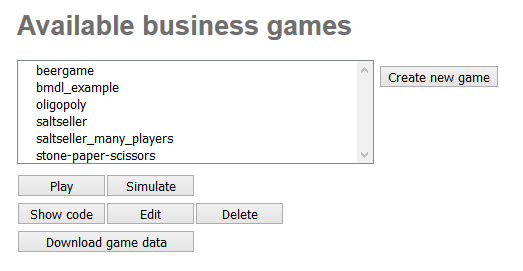
\includegraphics[scale=1]{figures/startpage.png}
	\caption{Startpage module}
	\label{fig:startpage}
\end{figure}

Figure \ref{fig:startpage} shows a realisation of the startpage module with all the business games that are currently available on the BGE implementation on \textit{http://games.fkmt.de}. The create, show, edit and delete buttons link to the development environment as described in section \ref{subsec:bge:d&a}. The other buttons link to the playing, simulation and analysis environment.

\subsection{Online editor and feedback screen}
\label{sub:module:editor}

The online editor module is used in the development, simulation and playing environment. In the development environment it enables to create new business games or to show or to edit the game code of existing games. In the simulation environment the editor displays the results or the errors of the simulation. In the playing environment it is optionally used if turned on in the source code in order to present game results to the players (below the charts).

The feedback screen is used for game validation in the development environment. It shows syntactic or semantic errors when creating or editing a game as described in section \ref{subsub:verification}. Figure \ref{fig:editor} shows the editor and feedback screen module displaying a semantic error.

\begin{figure}
	\centering
	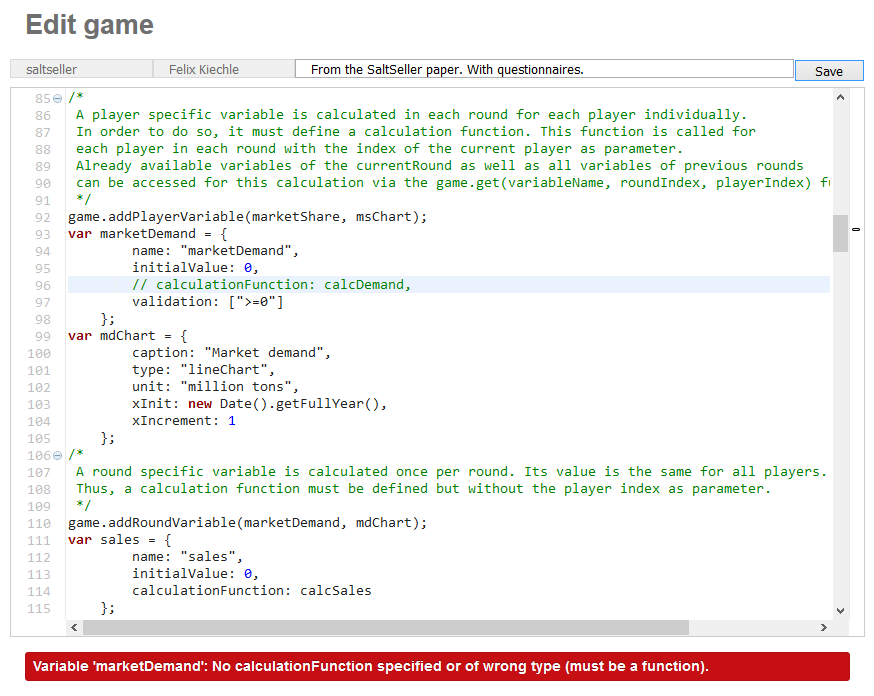
\includegraphics[scale=0.61]{figures/editor.png}
	\caption{Editor and feedback screen module}
	\label{fig:editor}
\end{figure}

The editor is based on the open-source Eclipse project \textit{Orion}\footnote{https://wiki.eclipse.org/Orion, retrieved on 03 Jan. 2016} which aims to create a browser based integrated development environment (IDE). It uses the open-source JavaScript parser \textit{Esprima}\footnote{https://http://esprima.org/, retrieved on 03 Jan. 2016} for the syntax analysis of the game code. Esprima is furthermore used together with the \textit{escodegen} project\footnote{https://github.com/estools/escodegen, retrieved on 03 Jan. 2016} for reformatting the source code after loading it from the database (show or edit). Reformatting is also used for the presentation of simulation results.

\subsection{Entrance hall and game engine}
\label{sub:module:engine}

The entrance hall and the game engine module enable game play and simulation as described in section \ref{subsec:bge:simplay}. The entrance hall is implemented so that the game starts automatically after the minimal number of players is reached and in such a way that $playerIDs = \{0,\dots, n-1\}$.

The game engine implements client-side game code execution. Table \ref{tab:engine} provides an overview of the WebSocket events on server and client and the corresponding actions they trigger. The list is nearly complete. It only misses the \textit{abort} event which is emitted by the client if a player disconnects from the game during game play (closes or refreshes the tab) or does not provide inputs within the maximal decision time. The server then marks the game as aborted in the corresponding Player object and uses default input values or the last input values submitted for the rounds to come in order to allow the other players to continue the game.

This implementation of the game engine module uses Google Charts\footnote{https://developers.google.com/chart/interactive/docs/gallery/piechart, retrieved on 20 Oct. 2015} for rendering Chart objects. Figure \ref{fig:play} shows an example game session of the \textit{SaltSeller} business game after two rounds have been played. Figure \ref{fig:questionnaire} gives an example of a questionnaire.

\begin{table}
	\centering
   \begin{tabular}{ p{7.825cm} | p{7.825cm}  }
      \textbf{Client} & \textbf{Server} \\
    \hline
      - Client connects and is asked to submit nickname \newline
      - \textbf{Emit event "play"}. Data: nickname and gamename &  \\
       ----------------------------------------------------->&  \textbf{On "play"}: \newline 
       - load gamecode from database \newline
       - Create Player object \newline
       - Join existing or create new game \newline
       - \textbf{Emit "wait join"} if minimal player number not yet reached \newline
       - Otherwise: \textbf{emitAll "init"} Data: game code, player objects\\
       \textbf{On "init"}: \newline
       - Instantiate new Game object \newline
       - Run game code \newline
       - Render input fields and questionnaires \newline
       - Wait for input or show questionnaire \newline
       - \textbf{Emit "input"} Data: inputs of all players or save questionnaire results to the Game object when user submits. & <-----------------------------------------------------\\
       ----------------------------------------------------->& \textbf{On "input"}: \newline
       - Save each incoming input data within the object that manages currently running games \newline
       - After all players have submitted input: \textbf{emitAll "calculate"} Data: input data of all players.\\
       \textbf{On "calculate"}: \newline
       - Create round object and write incoming input data to it \newline
       - Calculate round results (output variables) from inputs and write to round object \newline
       - Draw charts \newline
       - If last round: show game results, \textbf{emit "finish"} Data: whole Game object (contains complete game history) \newline
       - Not last round: increment round index, \textbf{emit "result"} Data: calculated round object&\\
       ----------------------------------------------------->&\textbf{On "result"}: \newline
       - NiceToHave: Fraud detection \newline
       - \textbf{Emit "set input"}\\
       &\textbf{On "finish"}: \newline
       - Save Game object to database \\
       \textbf{On "set input"}: \newline
       - Wait for input or show questionnaire \newline
       - \textbf{Emit "input"} Data: inputs of all players or save questionnaire results to the Game object after user submits.&<-----------------------------------------------------\\
      \hline  
    \end{tabular}
	\caption{Socket events on client and server }
    \label{tab:engine}
\end{table}

\begin{figure}
	\centering
	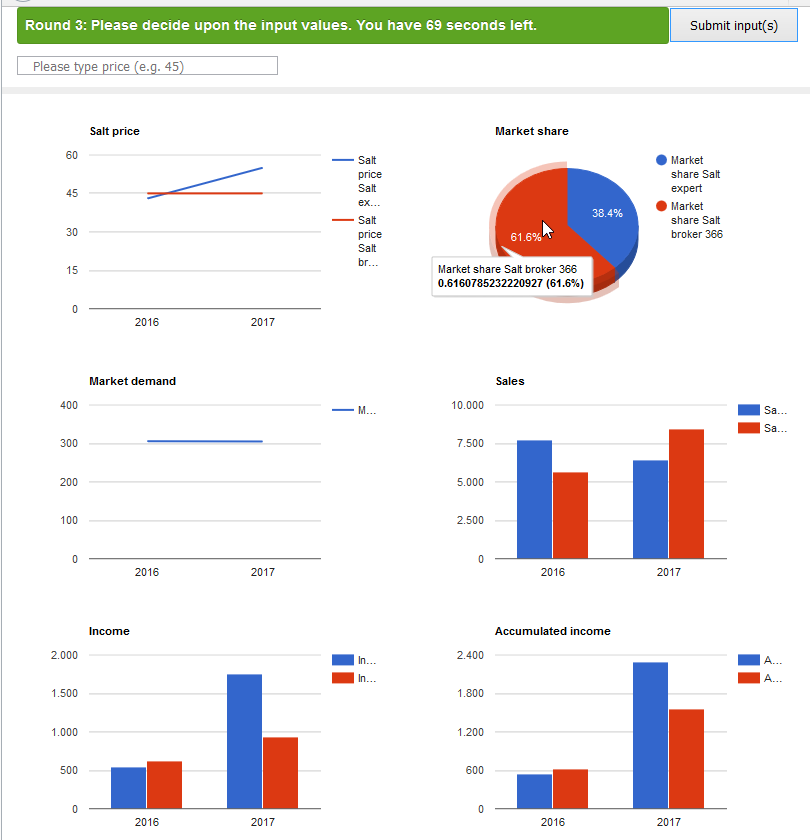
\includegraphics[scale=0.61]{figures/play.png}
	\caption{Screenshot of two players playing the \textit{SaltSeller} business game after two rounds have been played}
	\label{fig:play}
\end{figure}

\begin{figure}
	\centering
	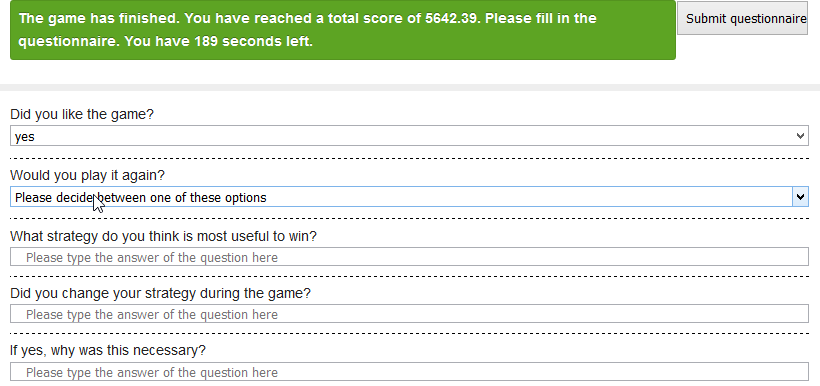
\includegraphics[scale=0.61]{figures/questionnaire.png}
	\caption{Example of a questionnaire which is displayed after the game has finished}
	\label{fig:questionnaire}
\end{figure}

\subsection{Game analysis}
\label{sub:module:analysis}

The entire game data of all game sessions of a specific business game which has been played on this instance of BGE can be downloaded as JSON file using the \textit{Download game data} button on the startpage. JSON is a well readable data exchange format (compared to XML for example) and libraries and utilities exist for all programming languages. 

Future implementations might provide an advanced analysis environment (see the next section) which can reduce the need for data analysts to learn the MongoDB query syntax or to write wrappers around the JSON files.
\newpage
\section{Dependencies}
Table \ref{table:dep} provides a brief overview of the third party libraries used in BGE.
\begin{table}
	\centering
    \begin{tabular}{ | p{5cm} | p{9,65cm} | }
    \hline 
    \textbf{Library} & \textbf{Description} \\
    \hline  
      Node.js \newline https://nodejs.org & Event-driven, non-blocking JavaScript Runtime for the server\\
      \hline  
      MongoDb \newline https://www.mongodb.org  & NoSQL database \\
      \hline 
      mongodb \newline https://www.npmjs.com/\newline package/mongodb 
      & MongoDb driver for Node.js \\
      \hline  
      express.js \newline 
      http://expressjs.com
      & Web server framework for Node.js \\
      \hline 
            socket.io \newline 
      http://socket.io
      & WebSocket implementation for Node.js \\
      \hline 
      esprima \newline 
     http://esprima.org/
      & Open-source JavaScript parser \\
      \hline 
            escodegen \newline 
    https://github.com/\newline estools/escodegen
      & JavaScript code generator (for reformatting) \\
      \hline 
                csurf, bodyparser, cookieparser & Middleware used by express.js for CSRF protection and body/url parsing \\
      \hline 
       jade & Template rendering engine for Node.js (used to insert CSRF tokens) \\
      \hline 
       Google charts  https://dev elopers.google.com/chart/ & JavaScript Chart API \\
      \hline 
    Eclipse orion & Editor for the web-browser \\
      \hline 
          JQuery & JavaScript frontend utilities \\
      \hline
    Foundation \newline http://foundation.zurb.com & CSS framework \\
      \hline
      
    \end{tabular}
    	\caption{BGE dependencies }
    	\label{table:dep}
\end{table}

\section{Installation guide}
\label{sec:imp:installation}

This section provides a brief installation guideline for a Debian based system (e.g. Ubuntu). 

\subsection{Prerequisites}
Install Node.js
\begin{itemize}
    \item \textit{sudo apt-get install npm} --> Installs the node package manager (NPM)
    \item \textit{sudo npm install -g npm} --> Updates NPM to the latest version
    \item \textit{sudo ln -s /usr/bin/nodejs /usr/local/bin/node} --> Syslink to the node environment, maybe only needed on Ubuntu
    \item \textit{sudo npm install -g n} --> install node binary manager \newline (https://www.npmjs.com/package/n)
    \item \textit{n stable} --> install the newest stable version of node
\end{itemize}
Install MongoDB
\begin{itemize}
    \item \textit{sudo apt-get install mongodb}
\end{itemize}

\subsection{BGE installation}

\begin{itemize}
    \item Checkout or copy BGE code to some local folder
    \item Go inside that folder
    \item \textit{npm install} --> Reads package.json in order to locally (inside BGE folder) install all the dependencies needed for BGE (see last section)
\end{itemize}

\subsection{Run it locally}
\begin{itemize}
    \item \textit{node server.js} --> Starts the BGE server, will listen on port 3000
    \item Start a browser, navigate to \textit{localhost:3000}
\end{itemize}
\subsection{Deployment}
Deployment of Node.js applications is quite straightforward. Set up / rent a linux server and follow the installation guidelines. Then:
\begin{itemize}
    \item use supervisor\footnote{https://github.com/petruisfan/node-supervisor} or forever\footnote{https://github.com/foreverjs/forever} or pm2 to watch the server process and keep it alive
    \item redirect all incoming traffic to e.g. port 3000 so that node need not run with privileges\footnote{sudo iptables -t nat -A PREROUTING -i eth0 -p tcp --dport 80 -j REDIRECT --to-port 3000} \footnote{http://stackoverflow.com/questions/16573668/best-practices-when-running-node-js-with-port-80-ubuntu-linode}
    \item more professional setups might consider Jenkins: \textit{https://jenkins-ci.org/}
\end{itemize}
